\chapter{Efficient Encoding, Decoding, and Indexing} \label{chap:coding}
The mappings described in the previous chapter are only one part of the process for associating geospatial data to cells of a 3D DGGS.
With geospatial data mapped to the domain of the grid system, the set of cells associated with the geometry of the data---and the indices of said cells---must be obtained.
As described earlier, this entire process is known as grid encoding.
Likewise, there needs to be a process to obtain the geometry of a cell (in grid space) from its index, so that the geometry can be mapped to the corresponding cell geometry in physical space.
This process is known as grid decoding.


Beyond encoding and decoding, there are also operations and queries done with a DGGS directly in grid space.
These operations often use algorithms for traversing the grid through neighbour, parent, and child relationships between cells.
Thus, queries that give these relationships for a given cell are another essential component of a fully functioning DGGS.


This chapter completes the 3D DGGS's described in the preceding chapters by providing encoding, decoding, and indexing operations for the SDOG modifications and grid extension method.
However, different types of geometry typically require their own encoding algorithms.
In this thesis, we focus on point encoding as it is the most fundamental, with the encoding of more complex geometries built off this operation.
While SDOG already has hierarchical coding algorithms~\cite{yu2009sdog, yu2009coding} that are trivially adapted to work with the modified grids, we derive constant time alternatives that work for both the conventional grid and our modifications.
For completeness, we also describe algorithms for performing neighbour, parent, and child queries.
For the grid extension method, we derive these operations in such a way as to ensure interoperability and consistency between the 3D and input DGGS.


The content of \cref{chap:7:extension} is taken from our \textit{IJGI} article~\cite{ulmer2020general}, with a slightly modified presentation.
We also provide additional details on layer operations that are not present in the original article.


\section{SDOG}
When first introduced by Yu and Wu, the authors proposed two indexing schemes for use with SDOG~\cite{yu2009coding}.
These schemes are both based on a modified Morton code (also known as a Z-order curve)~\cite{morton1966computer}; however, one is intended for indexing a single resolution whereas the other for the full cell hierarchy.
We focus on the hierarchical scheme, as grid \textit{systems} are the main focus of this thesis.


\begin{figure}[ht!]
	\centering
	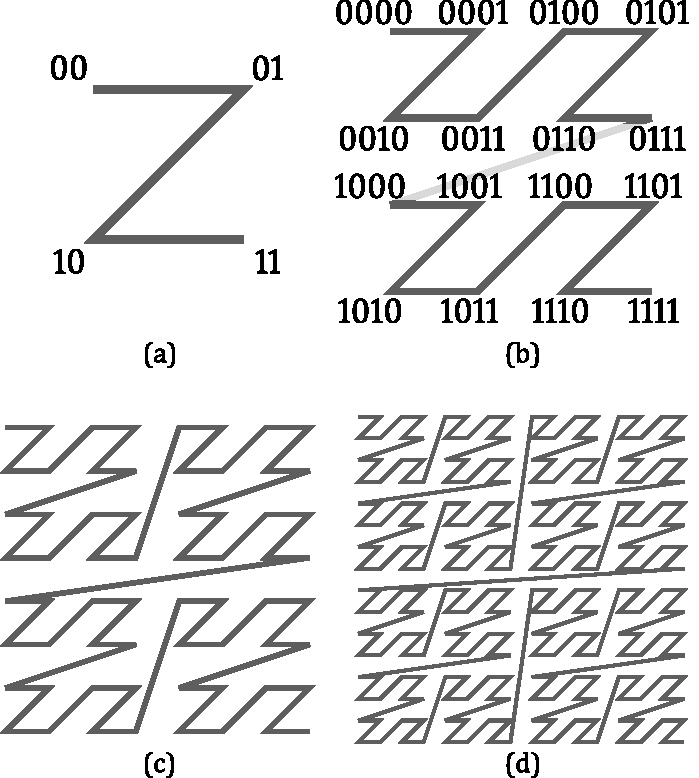
\includegraphics[width=0.6\textwidth]{morton-multiple.pdf}
	\caption[Four resolutions of Morton codes]{
		The first four resolutions of Morton codes for a quadtree.
		(a)--(d) show resolutions 1--4, respectively.
		Modified from~\cite{morton-multiple}; original image courtesy of David Eppstein -- CC BY-SA 3.0
	}
	\label{fig:morton-multiple}
\end{figure}


\Cref{fig:morton-multiple} demonstrates Morton coding for four resolutions of a conventional Euclidean quadtree.
Indices are assigned consecutively, starting at zero, to cells in the order the curve passes through them.
The resulting indices are hierarchical, where the index of a cell is that of its parent with its local index---obtained relative to its parent---appended.
While shown for a quadtree (2D), Morton codes generalize to any integer dimension $n$.
In this case, each cell has $2^n$ children, which means $n$ bits are needed to represent each uniquely.
Thus, from a given cell index, the resolution of the grid that cell appears at is the bit width of the index divided by $n$.
For a fixed-width representation of indices, a leaded bit set to one marks the start of the actual index.


\begin{figure}[htp!]
	\centering
	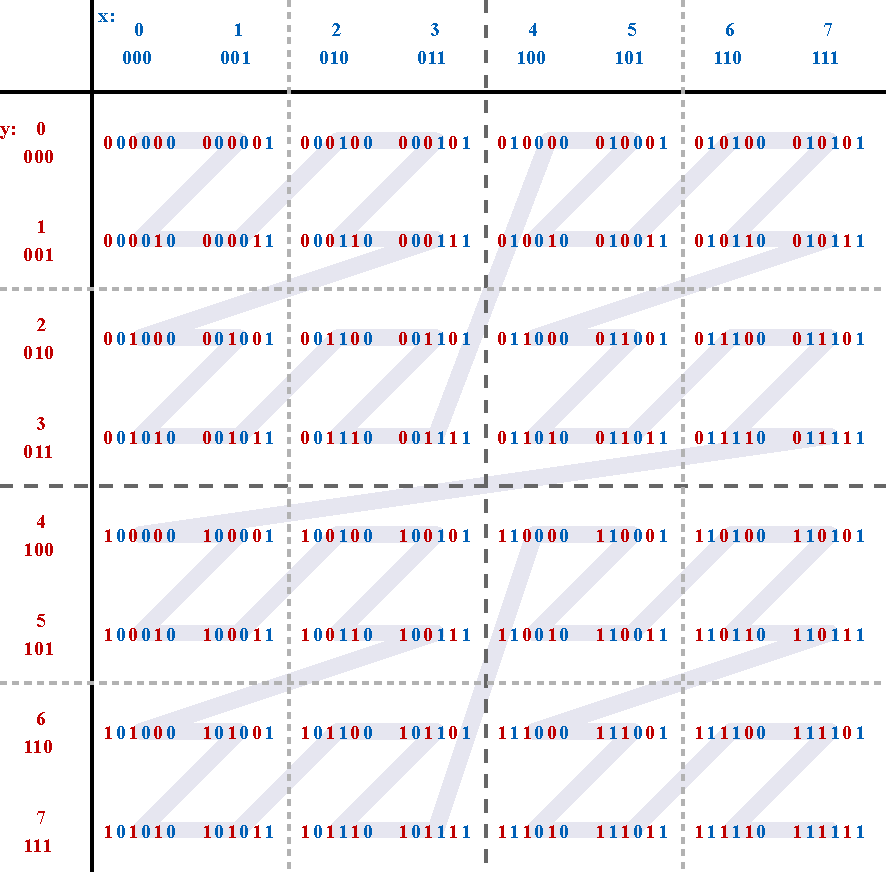
\includegraphics[width=\textwidth]{morton-interleave.pdf}
	\caption[Morton codes by bit-interleaving]{
		Third resolution Morton codes and their respective coordinate indices.
		Note how the Morton codes are obtained by interleaving the bits of the coordinate indices.
		In this figure, the $x$ coordinate is traversed first by the curve, so it is the lowest order bit in the Morton code.
		Image courtesy of David Eppstein~\cite{morton-interleave} -- CC BY-SA 3.0
	}
	\label{fig:morton-interleave}
\end{figure}


One benefit of Morton codes over more local space-filling curves---such as the Hilbert curve---is the ease at which a multi-dimensional index is encoded and vice versa.
As demonstrated in \cref{fig:morton-interleave}, the Morton code is obtained simply by interleaving the bits of the coordinate indices; likewise, unweaving the bits of a Morton code gives the coordinate indices.
While these are not constant-time operation in general, magic numbers and lookup tables allow them to be done efficiently and in constant time for a fixed bit width~\cite{libmorton18}.


\begin{figure}[ht!]
	\centering
	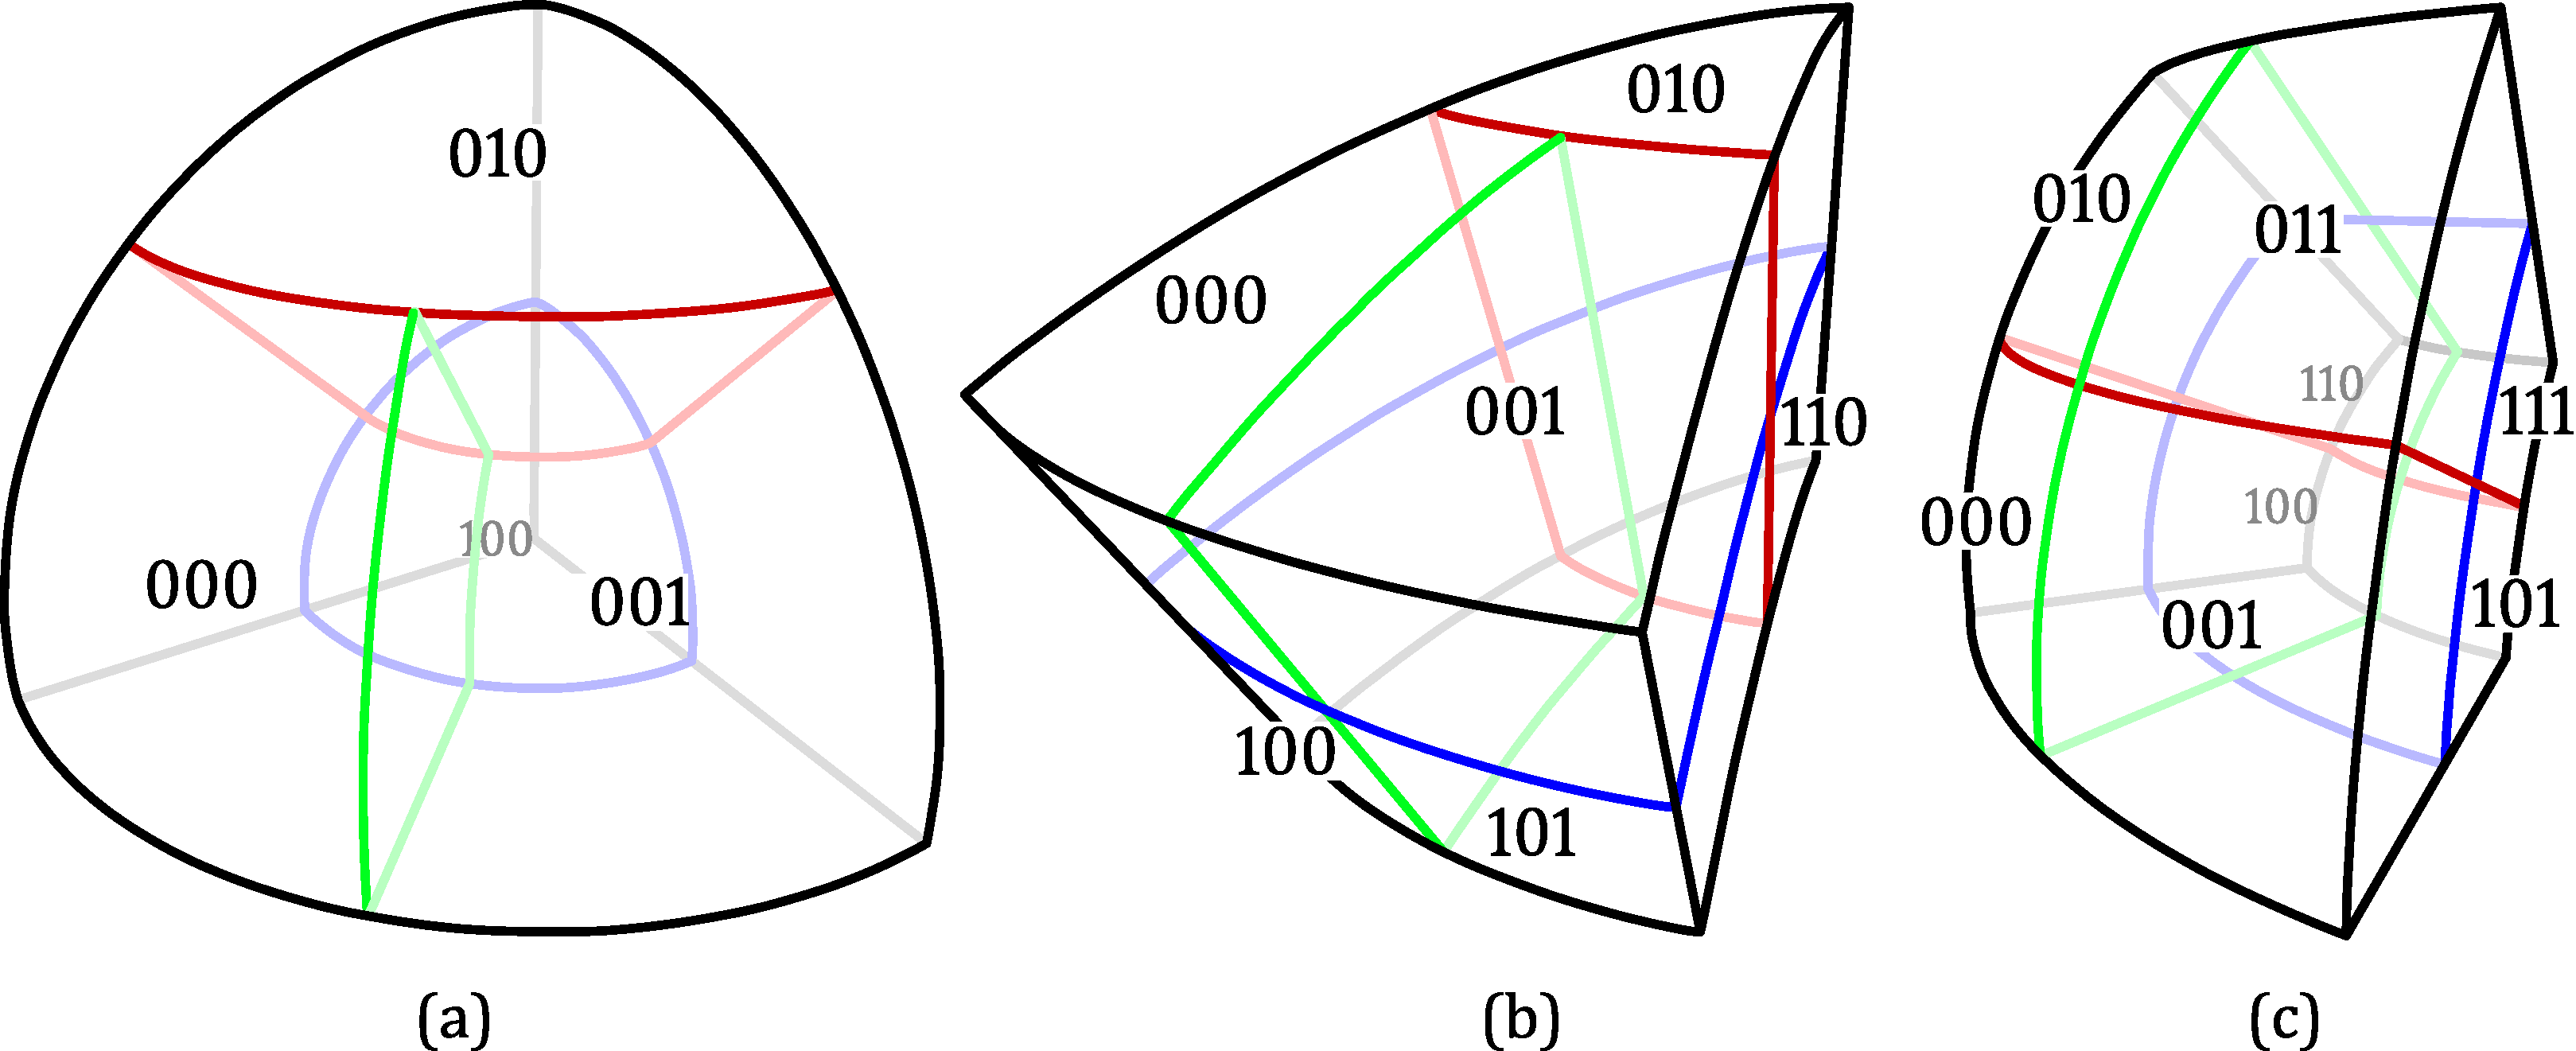
\includegraphics[width=\textwidth]{sdog-dmc.pdf}
	\caption[Degenerate Morton codes for the different SDOG cell types]{
		Degenerate Morton codes for (a) SG cells, (b) LG cells, and (c) NG cells.
	}
	\label{fig:sdog-dmc}
\end{figure}


While Morton codes have many desirable properties, due to the semiregular degenerate nature of SDOG, they must be modified for use with the grid system.
First, we apply Morton coding for a cell's children as if refinement was entirely regular.
For NG cells, refinement \textit{is} regular, and no modifications are needed.
However, for SG and LG cells, some of these codes will refer to the same cell.
In these cases, we merge duplicate codes with the lower value kept.
We call this the degenerate Morton code (DMC).
\Cref{fig:sdog-dmc} shows the child codes of cells for each SDOG cell type.
In this scheme, the different spherical coordinates are traversed in the order (1) longitude---small to large (2) latitude---small to large (3) radius---large to small.
Finally, to distinguish between the eight octants, each is given a unique identifier: the octant code.
The full index of an SDOG cell consists of the octant code and DMC, concatenated, along with a leading one for fixed-width representations.
For the remainder of this chapter, we assume the use of a fixed-width integer for representing SDOG indices.
From this definition, we know the number of bits needed to represent an SDOG index at refinement level $k$ is $3k + 4$.
Likewise, given an index with width $\omega$, the refinement level of that cell is $(\omega - 4) / 3$.
We use this property to implicitly obtain $k$ in any case where it is not provided.


\subsection{Hierarchical Algorithms}
We first give a brief overview of the hierarchical coding algorithms for SDOG, as these will be the baseline for evaluating our proposed ones.
Hierarchical coding works by traversing the grid system one resolution at a time, using the refinement rules for the relevant cell at each iteration.
As a result, these types of algorithms are linear on the level of refinement.
Furthermore, because they use refinement rules directly, they are trivially modified to work for our SDOG modifications by simply changing the refinement used in the algorithms accordingly.


\subsubsection{Encoding}
The algorithm for hierarchical point encoding with SDOG is given in \cref{alg:encode}.
The input is a point $p$ and resolution $k$; the output is the index $i$ of the cell that contains $p$ at $k$.


\begin{algorithm}
	\caption{Hierarchical point encoding for SDOG}
	
	\begin{algorithmic}
		
		\STATE determine which octant contains $p$
		\STATE cellBoundaries $\leftarrow$ boundaries of octant
		\STATE currCellType $\leftarrow$ SG
		\STATE $i \leftarrow \operatorname{append}(1, \mathrm{octantCode})$
		
		\FOR{$k$ iterations}
		\STATE use refinement rules for currCellType with cellBoundaries to find child cells
		\STATE determine which child contains $p$
		\STATE cellBoundaries $\leftarrow$ boundaries of child
		\STATE currCellType $\leftarrow$ type of child
		\STATE $i \leftarrow \operatorname{append}(i, \mathrm{child~index})$
		\ENDFOR
		\RETURN $i$
		
	\end{algorithmic}
	\label{alg:encode}
\end{algorithm}


\subsubsection{Decoding}
The algorithm for hierarchical decoding with SDOG is given in \cref{alg:decode}.
The input is an index $i$; the output is the cell boundaries of $i$.


\begin{algorithm}
	\caption{Hierarchical cell decoding for SDOG}
	
	\begin{algorithmic}
		
		\STATE determine octant from $i$
		\STATE cellBoundaries $\leftarrow$ boundaries of octant
		\STATE currCellType $\leftarrow$ SG
		\STATE remove highest four bits of $i$
		
		\FOR{$k$ iterations}
		\STATE use refinement rules for currCellType with cellBoundaries to find child cells
		\STATE $c \leftarrow$ highest three bits of $i$
		\STATE remove highest three bits of $i$
		\STATE determine which child cell matches $c$
		\STATE cellBoundaries $\leftarrow$ boundaries of $c$
		\STATE currCellType $\leftarrow$ type of $c$
		\ENDFOR
		\RETURN cellBoundaries
		
	\end{algorithmic}
	\label{alg:decode}
\end{algorithm}


\subsection{Direct Algorithms}
For a uniform grid, the coordinate indices of the cell that contain a point are obtained trivially in constant time.
Likewise, the maximum and minimum coordinates of a cell are also easily computed from a coordinate index.
For these operations, the necessary variables are the number of cells and the range of values in each coordinate dimension.
We also know that the semiregular regions of SDOG are uniform when using conventional refinement rules.
Thus, if we determine the relevant semiregular region and the needed properties of said region, we can apply direct coding algorithms for SDOG, with bit interleaving and unweaving giving the full DMC.


Under regular octree-based refinement, the number of cells in each coordinate direction is $2^k$.
Each increasing shell in SDOG halves the number of cells in the latitude and longitude coordinates.
Furthermore, each increasing zone further halves the number of cells in the longitude coordinate.
Since a DMC is relative to an octant, the range of coordinate values for direct coding are the ranges of the octant itself.
Therefore, all that we need for direct coding is the shell and zone that contain the point or cell being considered.


\subsubsection{Encoding}
The inputs and outputs of direct encoding are the same as their hierarchical counterpart.
First, we find the octant that contains $p$.
The three coordinates of $p$ are then normalized within the range of the octant with $\hat{r} = r / R_\mathrm{max}$, $\hat{\varphi} = \pm (2\varphi) / \pi$, and $\hat{\lambda} = 2 (\lambda - \lambda_0) / \pi$ where $\lambda_0$ is the minimum longitude of the octant.
We then calculate the shell and zone that contain $p$ the same as in \cref{chap:mapping}: $s = \lfloor \log_{0.5} \hat{r} \rfloor$ and $z = \lfloor \log_{0.5} ( 1 - \hat{\varphi} ) \rfloor$.


The number of latitude division is $2^k$ divided by $2^s$; however, the number of divisions will always be at least one.
Thus, we introduce variable $k_\varphi = \min ( s, k )$.
Similarly, the number of longitude division is $2^k$ divided by $2^{s+z}$, but again, will always be at least one.
We introduce a second variable $k_\lambda = \min ( s + z, k )$.


Finally, we calculate coordinate indices, making sure to account for the direction of each coordinate in the DMC for SDOG.
Let the subscript $i$ refer to the index the coordinate, then
%
\begin{equation*}
r_i = 2^k \cdot ( 1 - \hat{r} ),
\end{equation*}
%
\begin{equation*}
\varphi_i = 2^{k - k_\varphi} \cdot \hat{\varphi}, \quad \text{and}
\end{equation*}
%
\begin{equation*}
\lambda_i = 2^{k - k_\lambda} \cdot \hat{\lambda}.
\end{equation*}
%
The DMC, then, is the Morton interleaving of $\lambda_i$, $\varphi_i$, and $r_i$ (in that order); the full index is the octant code and DMC concatenated with the preceding bit set.


\subsubsection{Decoding}
The inputs and outputs of the direct decoding are the same as its hierarchical counterpart.
First, we get the octant code and DMC from $i$.
The DMC is then unwoven to get the coordinate indices $\lambda_i$, $\varphi_i$, and $r_i$.


We now decode the coordinate indices one at a time.
As the number of radial division is never modified, we start by decoding the radial index: 
%
\begin{equation*}
\hat{r}_\mathrm{max} = 1 - \frac{r_i}{2^k}, \quad \text{and}
\end{equation*}
%
\begin{equation*}
\hat{r}_\mathrm{min} = 1 - \frac{r_i + 1}{2^k}
\end{equation*}
%
With this, we can now determine the shell that contains the cell being decoded.
We use $\hat{r}_\mathrm{max}$ as opposed to $\hat{r}_\mathrm{min}$, as the latter gives the inner shell if on the boundary. Thus, $s = \lfloor \log_{0.5} \hat{r}_\mathrm{max} \rfloor$.
Just as with encoding, we define $k_\varphi = \min ( s, k )$.
We now have the needed information to decode latitude:
%
\begin{equation*}
\hat{\varphi}_\mathrm{max} = \frac{\varphi_i + 1}{2^{k - k_\varphi}}, \quad \text{and}
\end{equation*}
%
\begin{equation*}
\hat{\varphi}_\mathrm{min} = \frac{\varphi_i}{2^{k - k_\varphi}}.
\end{equation*}
%
Likewise, we can now determine the zone that contains the cell.
Opposite of radius, $\hat{\varphi}_\mathrm{max}$ now gives the higher zone if on the boundary, so we use $\hat{\varphi}_\mathrm{min}$ and get $z = \lfloor \log_{0.5} ( 1 - \hat{\varphi}_\mathrm{min} ) \rfloor$.
Again, the same as encoding, we define $k_\lambda = \min ( s + z, k )$.
Finally, we decode longitude:
%
\begin{equation*}
\hat{\lambda}_\mathrm{max} = \frac{\lambda_i + 1}{2^{k - k_\lambda}}, \quad \text{and}
\end{equation*}
%
\begin{equation*}
\hat{\lambda}_\mathrm{min} = \frac{\lambda_i}{2^{k - k_\lambda}}.
\end{equation*}
%
The last step is to get the bounds of the octant from the octant code and convert the normalized values to actual ones.


\subsubsection{For Modified SDOG}
These direct algorithms only work for conventional SDOG due to the requirement of uniform spacing of grid divisions.
As described in \cref{chap:mapping}, however, the mapping functions allow these algorithms to be used with the modified grids by mapping them to conventional SDOG.
For encoding, the point $p$ must be forward mapped before encoding.
For decoding, the output ranges must be inverse mapped after decoding.
In both cases, there is overlap in the computations done by the coding algorithm and associated mapping functions, so care should be taken during implementation to avoid redundant computation.


\subsection{Runtime Comparison}
To evaluate the usefulness of our direct coding algorithms, we should compare their runtime against the hierarchical counterparts.
To do so, we have implemented the four algorithms and the mapping functions presented in \cref{chap:mapping} in C++.
We also used these implementations to experimentally verify the correctness of the direct algorithms by comparing their output to the hierarchical ones.


The combination of two algorithmic approaches (hierarchical vs. direct) and four grids (SDOG and the three modifications in \cref{chap:sdog}) result in eight total algorithms to compare for both encoding and decoding.
For simplicity, we only benchmark the DMC portion of coding.
First, we generate one million points randomly distributed within an SDOG octant.
For each resolution being benchmarked, we then time each of the encoding algorithms using the generated points.
The resulting indices are then used to time each of the decoding algorithms in the same manner.
We time resolutions $1 \le k \le 21$, as 21 is the highest resolution \textit{without} an octant code that can be represented by a 64-bit integer.
We use the Libmorton library~\cite{libmorton18} to perform efficient bit-interleaving and unweaving.


\begin{figure}[htp!]
	\centering
	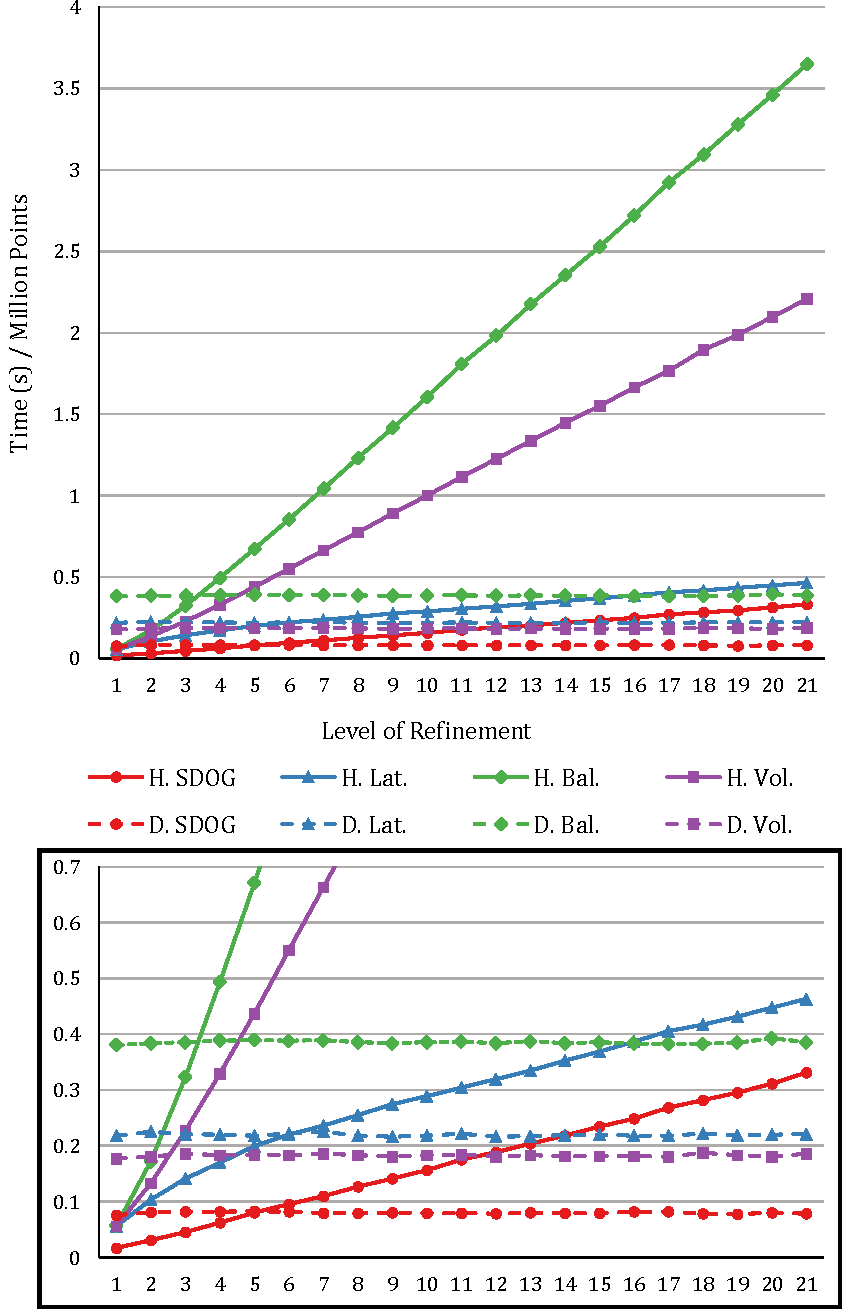
\includegraphics[width=0.8\textwidth]{point-to-index.pdf}
	\caption[Runtime comparison of SDOG point encoding algorithms]{
		Runtime of the hierarchical (H) and direct (D) encoding algorithms for SDOG and our proposed modifications (Lat = Latitude, Bal = Balanced, and Vol = Volume).
		The bottom chart is the same as the top but with a smaller vertical scale to better compare values.
	}
	\label{fig:point-to-index}
\end{figure}


\begin{figure}[htp!]
	\centering
	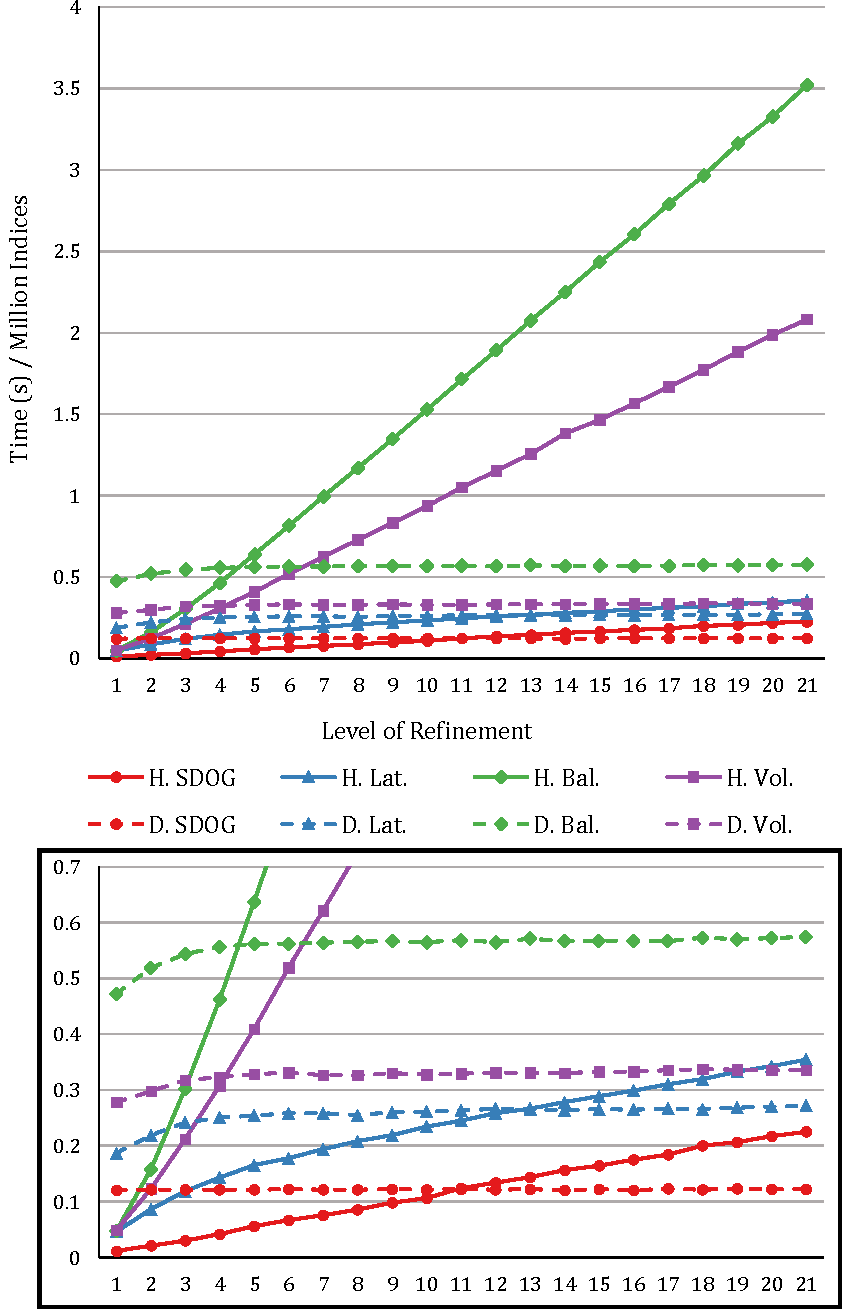
\includegraphics[width=0.8\textwidth]{index-to-range.pdf}
	\caption[Runtime comparison of SDOG decoding algorithms]{
		Runtime of the hierarchical (H) and direct (D) decoding algorithms for SDOG and our proposed modifications (Lat = Latitude, Bal = Balanced, and Vol = Volume).
		The bottom chart is the same as the top but with a smaller vertical scale to better compare values.
	}
	\label{fig:index-to-range}
\end{figure}


\Cref{fig:point-to-index,fig:index-to-range} show the benchmarking results for encoding and decoding, respectively.
In order to reduce noise, these charts show the average of two evaluations of the benchmarking.
As is expected, the hierarchical algorithms are linear on $k$ and the direct algorithms (mostly) constant on $k$.


For the hierarchical algorithms, the difference in runtime between the different grids is determined by the complexity of calculating splitting surfaces for cells.
For hierarchical encoding and decoding, SDOG is the most efficient closely followed by the latitude method; the volume method is significantly slower than these two, and the balanced method significantly slower than the volume one.
For the direct algorithms, this difference is determined by the complexity of evaluating the mapping functions.
For direct encoding, SDOG is most efficient, then volume closely followed by latitude, and then balanced.
Decoding is slightly different, with latitude and volume swapping places in the ordering.


In general, the hierarchical decoding algorithms are slightly quicker than their encoding counterparts.
The reasons for this are not entirely clear; however, it seems to imply that determining which child cell contains a point is slightly more expensive than setting the child cell dimensions based on a given code.
For the direct algorithms, the opposite holds, and the encoding algorithm is the quicker of the two.
The reason for this is the encoding algorithm only computes three values (an index for each coordinate), whereas the decoding must compute twice as many (a maximum \textit{and} minimum for each coordinate).
Furthermore, for the modified grids using the mapping functions, this means that decoding also requires twice as many uses of these functions.


Overall, the direct algorithms are all more efficient than their hierarchical counterpart for a large enough value of $k$.
Thus, a sophisticated implementation could determine which approach to use (hierarchical or direct) for a given input, depending on $k$.
However, benchmarking on a variety of platforms in different conditions would be needed to determine the best values to use for the switch.
\Cref{tab:hierarch-vs-direct} summarizes the lowest value of $k$ such that the direct algorithm is more efficient than the hierarchical for each pair of algorithms in \textit{our} benchmarking.


\begin{table}[htp!]
	\centering
	\caption[Resolution at which direct coding becomes more efficient than hierarchical]{
		The resolution ($k$) at which our direct coding algorithms become more efficient than their hierarchical counterparts
	}
	\begin{tabular}{@{} c c c c c @{}}
		\toprule
		         & SDOG & Latitude & Balanced & Volume \\ \midrule
		Encoding & 6    & 7        & 4        & 3      \\
		Decoding & 11   & 13       & 5        & 5      \\ \bottomrule
	\end{tabular}
	\label{tab:hierarch-vs-direct}
\end{table}


A final note is that runtime for direct decoding of the modified grids grows until about resolution four, where it then levels off to constant.
The reason for this is subtle.
In the decoding algorithm, values of $s$ and $z$ are calculated from the bounds of the cell being decoded.
Therefore, their values are bounded by $k$.
However, $s$ and $z$ are used as exponents when calculating $\ell$ and $u$ values, and in many implementations, calculating powers is faster for lower exponents (specifically, exponents of zero, one, and two).
Thus, low values of $k$ have lower maximum (and average) exponents and, therefore, slightly lower runtime.
This same effect does not appear in the encoding algorithms since $s$ and $z$ are calculated directly from $p$ with no respect to $k$.


\subsection{Other Indexing Operations}
Since the SDOG indexing described above is based on coordinate indices, grid traversal queries are mostly straightforward.
However, the nature of semiregular degenerate refinement introduces a few complications that make parent, child, and neighbour operations more complex than the respective operations in a perfectly regular grid.
We briefly describe how to perform each of these for a given SDOG index, $i$, below.


\paragraph{Parent}
The use of Morton interleaving makes parent queries trivial. The parent of $i$ is simply $i$ with the lowest three bits removed.


\paragraph{Children}
The children of an SDOG cell depend on the cell type.
A cell is SG if $r_i = 2^k - 1$, LG if $\varphi_i = 2^{k - k_\varphi} - 1$, and otherwise it is NG.
Let $C$ be the set of child codes for the cell type of $i$ (refer to Figure~X), then the children of $i$ are $\{ \operatorname{append}(i, c) \ | \ c \in C \}$


\paragraph{Neighbours}
Neighbours are by far the most complicated of the three operations due to the number of edge cases that need be handled.
First, we obtain the coordinate indices of $i$ just as with decoding.
In general, the coordinate indices of the neighbours of an SDOG cell are $\{ (\lambda_i', \varphi_i', r_i') \ | \ x' \in x \pm 1 \}$, which are then interleaved and combined with the octant code for the full index.
However, specific cells in SDOG require a modified formulation for certain neighbours.
Below we list how to detect these edge cases and how to modify the neighbour calculation accordingly.
%
\begin{enumerate}
	\item If $\lambda_i = 2^{k - k_\lambda} - 1$, then $\lambda_i + 1$ is in a neighbouring octant.
	For this neighbour, set $\lambda_i' = 0$ and use the octant code for the neighbouring octant.
	\item If $\lambda_i = 0$, then $\lambda_i - 1$ is in a neighbouring octant.
	For this neighbour, set $\lambda_i' = 2^{k - k_\lambda} - 1$ and use the octant code for the neighbouring octant.
	\item If $\varphi_i = 0$, then $\varphi_i - 1$ is in a neighbouring octant.
	For this neighbour, set $\lambda_i' = 0$ and use the octant code for the neighbouring octant.
	\item If $\varphi_i = 2^{k - k_\varphi} - 1 - 1$, $r_i = 2^k - 1$, or $r_i = 0$, then the cell is on the boundary of the octant with no neighbours in the corresponding direction (increasing, increasing, and decreasing, respectively).
	\item If $\varphi_i = 2^n - 1$ for some $n \in \mathbb{Z}$, then $\varphi_i + 1$ is in the next spherical zone, which has half as many longitude divisions.
	For this neighbour, set $\lambda_i' = \lfloor \lambda_i / 2 \rfloor$.
	\item If $\varphi_i = 2^n$ for some $n \in \mathbb{Z}$, then $\varphi_i - 1$ is in the previous spherical zone, which has twice as many longitude divisions.
	In this case, there are two neighbours in this direction; set $\lambda_i' = 2 \lambda_i, \  2 \lambda_i + 1$.
	\item If $r_i = 2^n - 1$ for some $n \in \mathbb{Z}$, then $r_i + 1$ is in the next spherical shell, which has half as many longitude and laitude divisions.
	For this neighbour, set $\lambda_i' = \lfloor \lambda_i / 2 \rfloor$ and $\varphi_i' = \lfloor \varphi_i / 2 \rfloor$.
	\item If $r_i = 2^n$ for some $n \in \mathbb{Z}$, then $r_i - 1$ is in the previous spherical shell, which has twice as many longitude and latitude divisions.
	In this case, there are four neighbours in this direction; set $\lambda_i' = 2 \lambda_i, \  2 \lambda_i + 1$ and $\varphi_i' = 2 \varphi_i, \  2 \varphi_i + 1$.
\end{enumerate}
%


\section{Extension Method} \label{chap:7:extension}
For our grid extension method, encoding and decoding operations are defined for the input DGGS and should be leveraged when defining the 3D version of these operations.
Doing so not only simplifies the definition of these operations (by deferring work to the input DGGS) but also facilitates the simple transference of data between the input DGGS and its 3D counterpart.
To accomplish this, we split encoding and decoding into a surface and radial component.
Referring to \cref{fig:prismatoid-indexing}, we justify such a split by noting that two components define each cell in a 3D DGGS: the cell of the input DGGS that defines its base(s) and the layer of the grid that contains it.
Uniquely identifying each of these components is sufficient to identify every cell in the grid uniquely; furthermore, each of these components is determined almost entirely independently.


\begin{figure}[htp!]
	\centering
	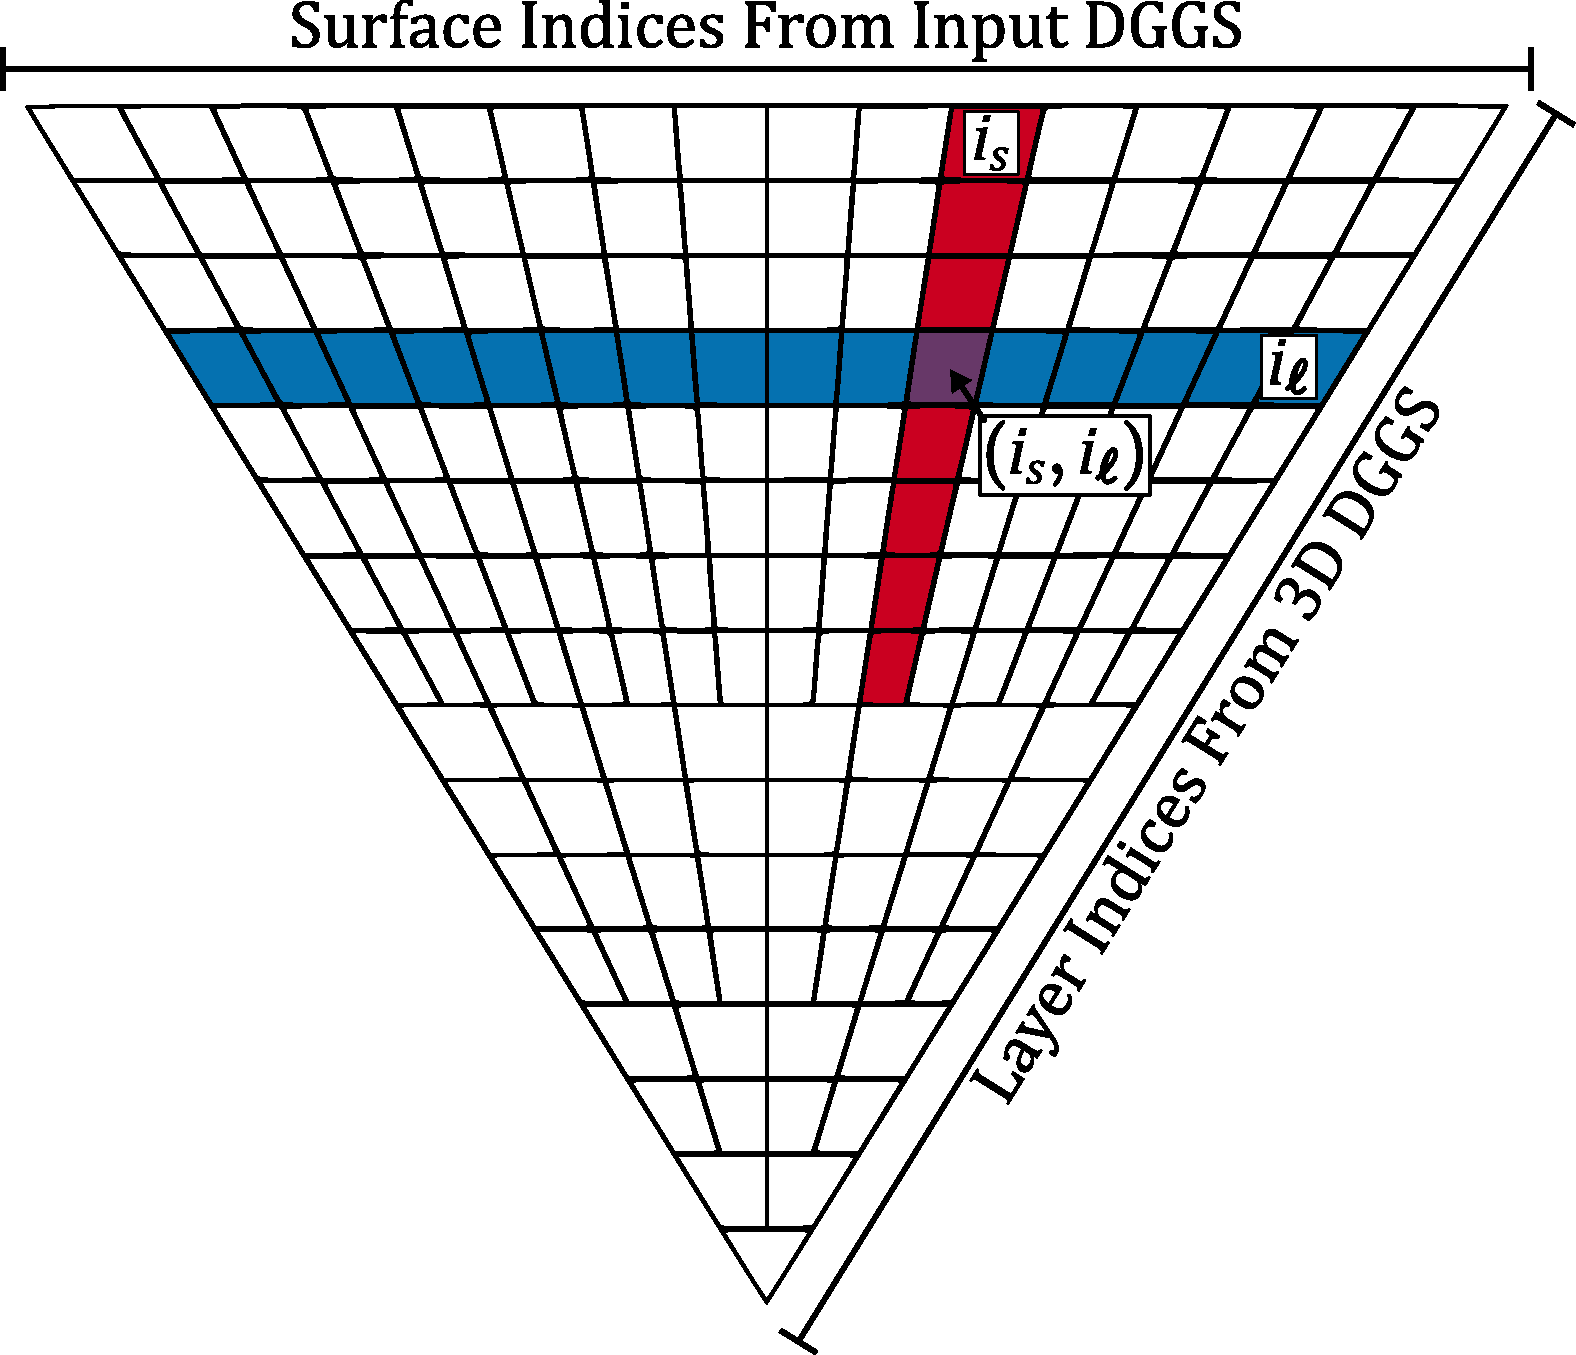
\includegraphics[width=0.6\textwidth]{prismatoid-indexing.pdf}
	\caption[Separation of surface and layer indices for the grid extension method]{
		Indices from the input DGGS identify cells in the 3D DGGS with the same bases but different radii.
		Likewise, each layer of the 3D DGGS contains all cells with the same radii but different bases.
		Thus, these two pieces of information combined are sufficient to identify any cell in the 3D DGGS uniquely.
		Here we show a single cell---highlighted in purple---along with all the cells that share a surface index (red) and a layer index (blue)
	}
	\label{fig:prismatoid-indexing}
\end{figure}


\Cref{fig:prismatoid-coding} illustrates the pipeline for our proposed split of these operations.
The surface component of coding is handled entirely by the input DGGS and, therefore, is not discussed here.
For the radial component, encoding and decoding make use of the forward and inverse radial mapping functions provided in \cref{chap:6:radial}, respectively.
We also provide a parameterization for identifying the layers of a 3D DGGS, and operations for encoding and decoding this parameterization.
We do \textit{not} discuss methods for converting this parameterization into a single index or for combining surface and layer indices into a single index (nor do we provide the inverse for either of these operations).
For the former, the varying complexity of the layer structure in a 3D DGGS---combined with the competing goals of an indexing scheme---makes defining a general method for doing so challenging.
For the latter, this operation depends heavily on the input DGGS and layer indexing and cannot be easily defined in general.


\begin{figure}[htp!]
	\centering
	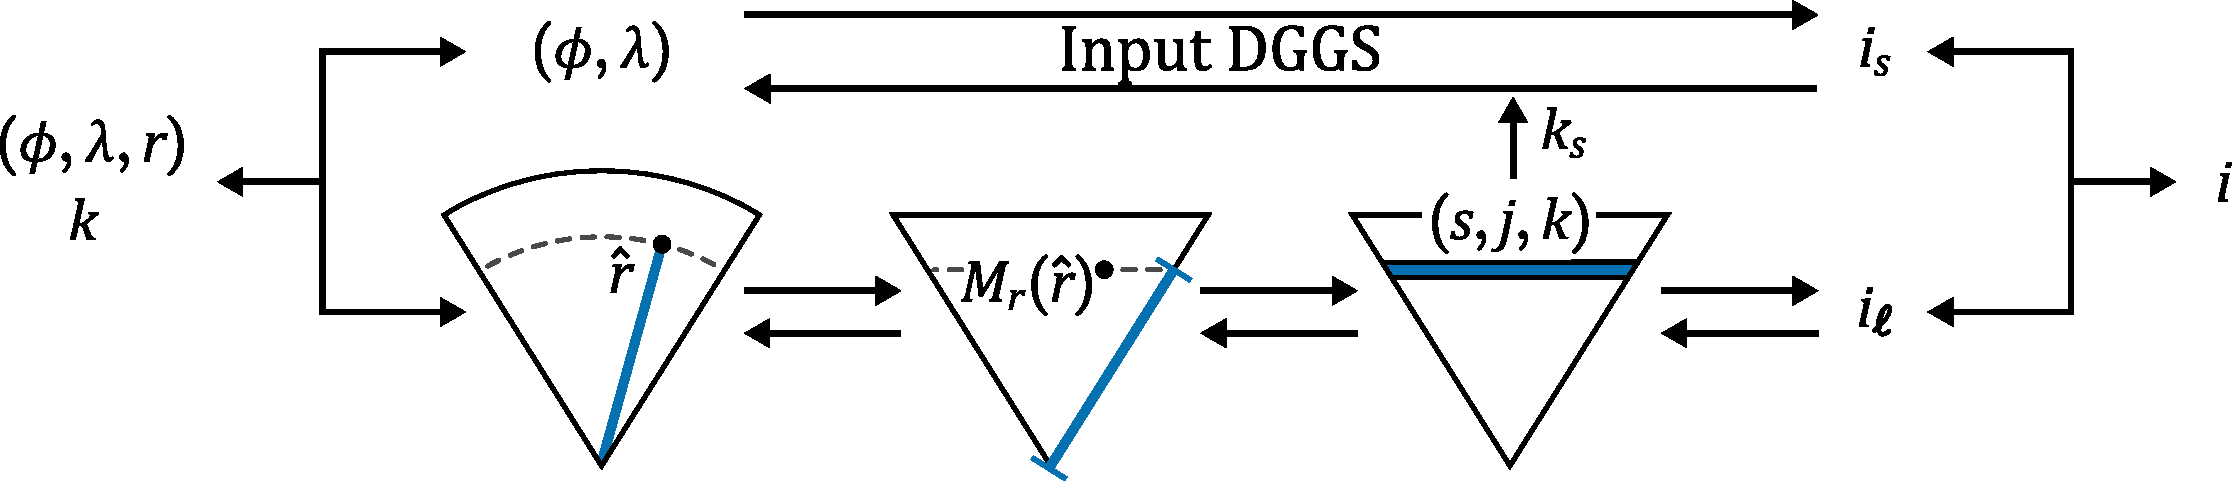
\includegraphics[width=\textwidth]{3d-coding.pdf}
	\caption[Pipeline for encoding and decoding with the grid extension method]{
		Pipeline for splitting encoding and decoding into surface (top) and radial (bottom) components.
		These two components are entirely independent except for the surface resolution ($k_s$) of the layer being provided to the surface component during encoding
	}
	\label{fig:prismatoid-coding}
\end{figure}


Layers of our 3D DGGS's can be parameterized by the shell they reside in ($s$), the integer index of the layer relative to the shell ($j$), and the level of refinement ($k$); we denote the central layer with $s = -1$.
Thus, layer encoding will calculate these values from $\hat{r}$ and layer decoding will calculate $\hat{r}_\mathrm{max}$ and $\hat{r}_\mathrm{min}$ from these values.


\subsection{Encoding}
The level of refinement $k$ is an input into encoding; therefore, only $s$ and $j$ need to be computed.
The value of $s$ is carried forward from the radial mapping function evaluation.
In order to calculate $j$, the number of layers in the shell is first needed; this depends on the refinement level, the layering sequence, and the number of extra radial splits (see \cref{chap:extension}).
The refinement level is an input, and the other variables are constant for any given 3D DGGS.
The number of layers is
%
\begin{equation*}
n_\ell = \left( x+1 \right) \prod_{i = s}^{k - 1} \ell_i.
\end{equation*}
%
Recall that $\ell_i$ refers to the number of layer produced when refining normal layers at refinement level $i$, which is unrelated to the values $\ell_g$ and $\ell_p$.
In the case where $s$ is greater than $k-1$, the shell is in the central layer.
In this case, we set $s = -1$ and $j = 0$.
The integer index of the layer is then $j = \lfloor d \cdot n_\ell \rfloor$, where $d$ is carried forward from the radial mapping function.
Finally, as input into the surface encoding, the value of $k_s$ is needed for the shell.
For central layers, this is always zero; otherwise, it is $k - s - 1 + w$.


Note that only the values of $s$ and $d$ are used in the above calculation and \textit{not} $\hat{r}$.
Therefore, the full evaluation of the radial mapping is unnecessary, and only \cref{eq:radialForwD} is evaluated for encoding.


\subsection{Decoding}
For decoding, we calculate $d_\mathrm{min}$ and $d_\mathrm{max}$ as $j/n_\ell$ and $(j+1)/n_\ell$, respectively.
These values are then fed directly into the inverse radial mapping as values of $d$ in \cref{eq:radialInv}.


\subsection{Other Indexing Operations}
Similar to encoding and decoding, we define grid traversal operations in terms of surface and radial components.
Referring back to \cref{fig:prismatoid-indexing,fig:prismatoid-coding}, we let $i_s$ be the surface index of a cell and $i_\ell$ be the layer index.
For each of these components, we assume there is a corresponding parent(s), child, and neighbour operation.
For the surface index, this comes directly from the input DGGS indexing, whereas for the layer index, we define these in terms of the layer parameterization provided above.


\subsubsection{Layer Operations}
For each of the operations, we describe how to calculate the output layer parameterization(s) $(s',j',k')$ from that of the input layer $(s,j,k)$.


\paragraph{Parent}
Trivially, the parent layer is in the previous resolution of the 3D DGGS, so $k' = k - 1$.
For calculating $s$ and $j$, there are two cases, which correspond with the parent layer being central or normal.
If $s = k-1$ or $s = -1$, then the parent layer is a central layer. In this case, $s' = -1$ and $j' = 0$.
Otherwise, the parent layer is normal with $s' = s$ and $j' = \lfloor j / \ell_k \rfloor$.


\paragraph{Children}
The child layers depend on if the layer in question is central or normal.
Regardless, in both cases all children will have $k' = k + 1$.
Recall that $s = -1$ denotes that a given layer is central.
In this case, one child is the child central layer with $s' = -1$ and $j = 0$.
There are also a number of child normal layers equal to one plus the number of extra radial splits ($x$), given by $s' = s = k$ and $j' = \{ o \in \mathbb{Z} \ | \ o \in [0, x] \}$.
For normal layers, the children are found with $s' = s$ and $j' = \{ j \cdot \ell_k + o \ | \  o \in \mathbb{Z}, \ o \in [0, \ell_k - 1] \}$.


\paragraph{Neighbours}
Neighbour layers are the layers above and below a given layer; they are at the same resolution, so $k' = k$.
In most cases, the two neighbours are simply $s' = s$ and $j' = j \pm 1$; however, there are three edge cases that need to be handled.
If $j = n_\ell - 1$, then the layer above is $s = s - 1$ and $j = 0$; if $s - 1$ is negative then the layer is on the boundary of the grid and there is no layer above it.
If $j = 0$ then the layer below is $s' = s + 1$ and $j = n_\ell$, where $n_\ell$ is calculated with respect to the new shell (i.e. $s'$).
Finally, the central layer ($s = -1$) has no layer below it and the layer above it is $s' = k - 1$ and $j = 0$.


\subsubsection{Combined Operations}
With the surface and layer operations defined, we now give the full 3D ones.


\paragraph{Parents}
The parent(s) of a cell depends on if its layer and its parent layer have the same or different values of $k_s$.
Let $i_\ell' = \operatorname{parent}(i_\ell)$; if the value of $k_s$ is the same, then the single parent is simply $(i_s, i_\ell')$.
In most cases, the value of $k_s$ for $i_\ell'$ is some number $m$ (often one, but not always) less than that of $i_\ell$.
In this case, the parent(s) are given by $\operatorname{parents}^m(i_s) \times i_\ell$.


\paragraph{Children}
The children of a cell depend on if the cell belongs to a central or normal layer.
For normal layers, the set of children is simply $\operatorname{children}(i_s) \times \operatorname{children}(i_\ell)$.
For central layers, the child who belongs to the new central layer must be distinguished from the other child layer(s).
Call the index of the new central layer $c_\ell$; then, this child is given by $(i_s, c_\ell)$.
Let $ N_\ell$ give the set of the other children layer indices (normal layers).
These layers have the surface refinement applied $w$ times, so the resulting children are $\operatorname{children}^w(i_s) \times N_\ell$.


\paragraph{Neighbours}
We split neighbours into three categories: neighbours in the same layers as the cell, neighbours in the layer above the cell, and neighbours in the layer below the cell.
If a cell belongs to the outermost or innermost (central) layer, then it will not have neighbours in the layer above or below, respectively.
Neighbours in the same layer are simply $\operatorname{neighbours}(i_s) \times i_\ell$.
Let $i_\ell^+$ be the layer above $i_\ell$ and $i_\ell^-$ be the layer below.
If $i_\ell^+$ has the same value of $k_s$ as $i_\ell$, then the single neighbour above is $(i_s, i_\ell^+)$.
In the other case, where the value of $k_s$ for $i_\ell^+$ is some number $m$ greater than that of $i_\ell$, the neighbours are given by $\operatorname{children}^m(i_s) \times i_\ell^+$.
Likewise, if $i_\ell^-$ has the same value of $k_s$ as $i_\ell$, there is one neighbour below given by $(i_s, i_\ell^-)$.
In the case that the value of $k_s$ for $i_\ell^-$ is some number $m$ less than that of $i_\ell$, the neighbours are given by $\operatorname{parents}^m(i_s) \times i_\ell^-$.


\section{Summary}
Several critical operations enable the integration, analysis, and visualization of data in a DGGS.
By providing point encoding, cell decoding, and grid traversal queries for the 3D DGGS's presented earlier in the thesis, we allow them to serve as fully functioning grid systems.
While there exist more advanced DGGS operations, the ones discussed in this chapter are the most fundamental and operate as a key component in defining more complex queries and analysis.
For our modifications to SDOG, the combination of the mapping functions derived in \cref{chap:mapping} and our direct encoding and decoding algorithms allow for efficient constant-time performance of these operations.
This improved efficiency is especially noticeable at high refinement levels for the balanced and volume methods, where the direct approaches are an order of magnitude faster than their hierarchical counterparts.
For the grid extension method, the operations we provide are completely general and work for any valid 3D DGGS resulting from the method.
For a specific 3D DGGS, such generality may not be necessary.
In this case, more specific versions of these algorithms---with unnecessary calculations removed---should be derived and used instead.
